\documentclass[notheorems]{beamer}
%
% Choose how your presentation looks.
%
% For more themes, color themes and font themes, see:
% http://deic.uab.es/~iblanes/beamer_gallery/index_by_theme.html
%
\mode<presentation>
{
  \usetheme{default}      % or try Darmstadt, Madrid, Warsaw, ...
  \usecolortheme{beaver} % or try albatross, beaver, crane, ...
  \usefonttheme{structuresmallcapsserif}  % or try serif, structurebold, ...
  \setbeamertemplate{navigation symbols}{}
  \setbeamertemplate{caption}[numbered]
} 

%\usepackage{babel}
%\usepackage[utf8x]{inputenc}
\usepackage{CJKutf8}
\usepackage{multirow}
\usepackage{natbib}
\bibliographystyle{abbrvnat}
\usepackage[ruled]{algorithm2e}
\usepackage{booktabs}
\usepackage{subcaption}
\usepackage{xcolor} % http://www.ctan.org/tex-archive/macros/latex/contrib/xcolor
\usepackage{tikz}
\usetikzlibrary{fit,calc}
%define a marking command
\newcommand*{\tikzmk}[1]{\tikz[remember picture,overlay,] \node (#1) {};\ignorespaces}
%define a boxing command, argument = colour of box
\newcommand{\boxit}[1]{\tikz[remember picture,overlay]{\node[yshift=3pt,fill=#1,opacity=.25,fit={(A)($(B)+(.95\linewidth,.8\baselineskip)$)}] {};}\ignorespaces}
%define some colours according to algorithm parts (or any other method you like)
\colorlet{pink}{red!40}
\colorlet{blue}{cyan!60}

\renewcommand{\refname}{参考文献}
\renewcommand{\figurename}{图}
\renewcommand{\tablename}{表}
\renewcommand*{\algorithmcfname}{算法}
\SetKwInput{KwIn}{输入}
\SetKwInput{KwOut}{输出}
\newcommand{\R}{\mathbb{R}}
\newcommand{\N}{\mathbb{N}}
\newcommand{\E}{\mathbb{E}}
\DeclareMathOperator*{\argmax}{argmax}
\DeclareMathOperator*{\argmin}{argmin}
\newcommand{\norm}[1]{\left\lVert#1\right\rVert}
\newtheorem{theorem}{定理}
\newtheorem{lemma}[theorem]{引理}
\newtheorem{definition}{定义}

\title{面向大数据的扁平聚类算法研究}
%references:
%https://tex.stackexchange.com/questions/280713/creating-author-blocks-in-beamer-using-authblk-package
%https://cn.sharelatex.com/learn/Beamer
\author{任远航 \\ 201721220117 \\ \texttt{ryuanhang@gmail.com}}
\institute{信息与软件工程学院 \\ 电子科技大学}
\date{2020年5月8日}

\begin{document}
\begin{CJK*}{UTF8}{gbsn}
% make title page
\begin{frame}
  \titlepage
\end{frame}

% Uncomment these lines for an automatically generated outline.
% \begin{frame}{Outline}
%  \tableofcontents
% \end{frame}
\AtBeginSection[]
{
  \begin{frame}
    \frametitle{目录}
    \tableofcontents[currentsection] 
  \end{frame}
}
\AtBeginSubsection[]
{
	\begin{frame}
		\frametitle{目录}
		\tableofcontents[ 
		sectionstyle=show/hide,
		subsectionstyle=show/shaded/hide, 
		] 
	\end{frame}
}

\section{介绍}

\begin{frame}{聚类}

\begin{itemize}
  \item 什么是聚类?
%   reference:
%   https://stackoverflow.com/questions/144639/how-to-order-citations-by-appearance-using-bibtex
% 	https://tex.stackexchange.com/questions/103192/cite-author-and-number-index
% 	https://tex.stackexchange.com/questions/340056/cite-and-footnote-in-together-in-beamer
% 	https://tex.stackexchange.com/questions/315627/how-to-cite-a-reference-on-beamer-as-author-year/315632
  \item 扁平聚类vs层级聚类
\end{itemize}

\begin{figure}
\centering
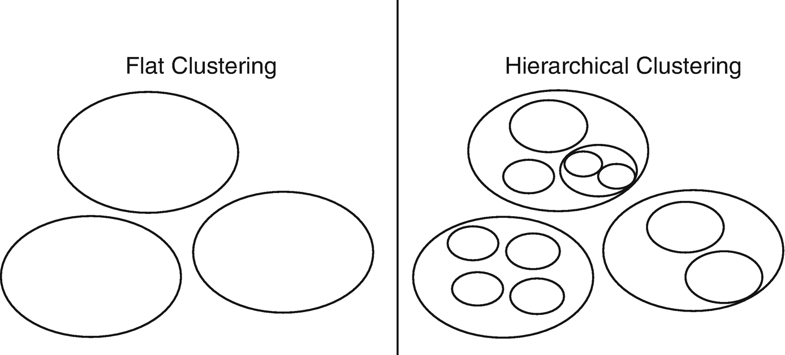
\includegraphics[scale=0.2]{clustering_types.png}
\end{figure}

\end{frame}

\begin{frame}{研究的问题}
大数据下满足下列条件的算法是急需的:
\begin{itemize}
	\item 有理论保证
	\item 高效
\end{itemize}
本论文将围绕$k$-means和谱聚类展开研究
\end{frame}

\section{$k$-means}

\subsection{背景}

\begin{frame}{$k$-means问题}

\begin{itemize}
	\item 得益于Lloyd算法 \citep{lloyd1982least},这一问题非常有名
	\item $k$-means问题是NP难的
\end{itemize}
\begin{definition}[$k$-means问题]
	给定数据集$\mathcal{X} \subseteq \R^d$以及$k$个点的集合$C \subseteq \R^d$,定义如下目标函数
	\begin{equation}
		\phi_C(\mathcal{X}) = \sum_{x \in \mathcal{X}}d^2 (x,C)
	\end{equation}
	其中$d(x,C) = \min\limits_{c \in C}\norm{x - c}$是点到集合的距离,$k$-means问题的目标是找到最优的$C$从而使得上式最小
\end{definition}

\end{frame}

\begin{frame}{解的质量}
	\begin{definition}[解的质量1]
		令$\alpha \geq 1$,如果下式成立,称$C$是$k$-means问题的一个$\alpha$近似解
		\begin{equation}
		\phi_C(\mathcal{X}) \leq \alpha \phi_\text{OPT}(\mathcal{X})
		\end{equation}
		其中$\phi_\text{OPT}(\mathcal{X})$是最优距离平方和
	\end{definition}
	\begin{definition}[解的质量2]
		令$\alpha \geq 1$且$\beta > 0$,如果下式成立,称$C$是$k$-means问题的一个$\beta$-bad $\alpha$近似解
		\begin{equation}
		\phi_C(\mathcal{X}) > (\alpha + \beta)\phi_\text{OPT}(\mathcal{X})
		\end{equation}
		否则,$C$被称为$\beta$-good $\alpha$近似解
	\end{definition}
\end{frame}

\subsection{有理论保证的算法}

\begin{frame}{$k$-means++}
	$k$-means++ \citep{arthur2007k}利用\textit{$d^2$ weighting}得到了一个$O(\log k)$的近似解
	% ref: https://tex.stackexchange.com/questions/220589/how-to-scale-algorithm-to-fit-in-one-frame-and-centered-in-the-frame-at-same-tim
	
	\scalebox{0.8}{
		\begin{minipage}{0.7\linewidth}
			\begin{algorithm}[H]
				\caption{$k$-means++ seeding}
				\KwIn{数据集$\mathcal{X}$,类数目$k$}
				\KwOut{$k$个点$C$}
				$c_1 \gets $ 从$\mathcal{X}$中均匀采样一个点 \\
				$C \gets \{c_1\}$ \\
				\For{$i = 2,3, \ldots k$}{
					\For{$x \in \mathcal{X}$}{
						% we can calculate a small set of p instead of whole p(x)
						$p(x) \gets \text{d}(x,C)^2/\sum_{x' \in \mathcal{X}} \text{d}(x',C)^2$
					}
					$x \gets$依分布$p$从$\mathcal{X}$中采样一个点  \\
					$C \gets C\cup\{x\}$
				}
				\textbf{返回} $C$
			\end{algorithm}
		\end{minipage}
	}%
	\begin{minipage}{0.3\linewidth}
		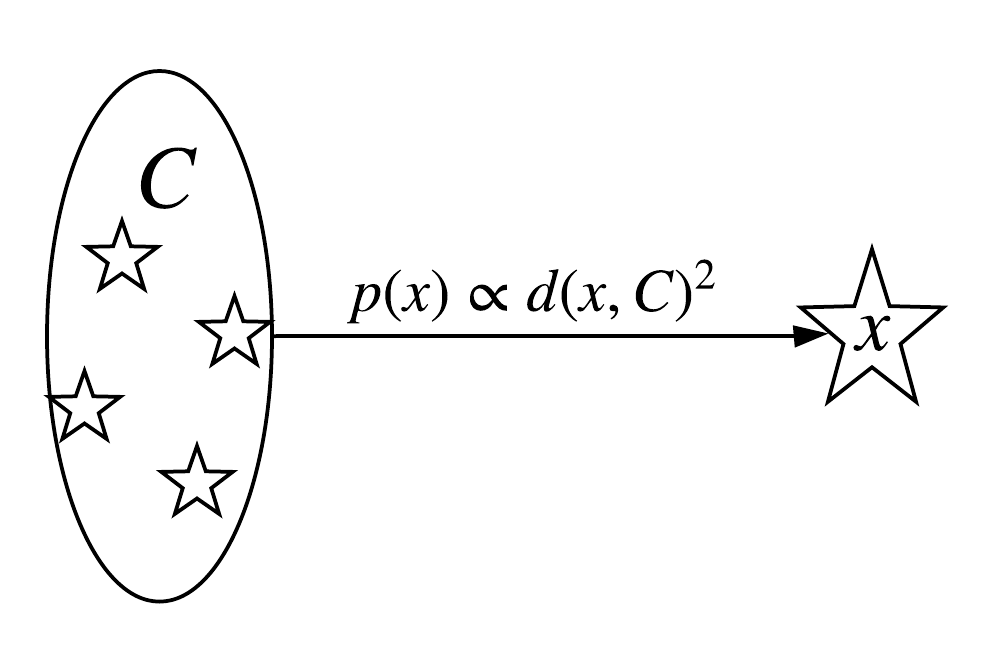
\includegraphics[scale=0.5]{kmeans++.png}
	\end{minipage}

\end{frame}

\begin{frame}{$k$-means\(\vert \vert\)}
	
	$k$-means\(\vert \vert\) \citep{bahmani2012scalable}加速了$k$-means++
	
	\scalebox{0.65}{
		\begin{minipage}{0.91\linewidth}
			\begin{algorithm}[H]
				\caption{$k$-means\(\vert \vert\) seeding}
				\KwIn{数据集$\mathcal{X}$,每一轮期望采样数$l$,聚类数$k$,轮数$t$}
				\KwOut{$k$个点$C$}
				$S \gets$ 从$\mathcal{X}$中均匀采样一个点\\
				\For{i = 1,2,...,t}{
					$C' \gets \emptyset$ \\
					\For{$x \in \mathcal{X}$}{
						以概率$\min(1,\frac{ld^2 (x,S)}{\phi(\mathcal{X},S)})$将$x$加入 $C'$中
					}
					$S \gets  S \cup C'$
				}
%				ref: https://tex.stackexchange.com/a/386274
				\tikzmk{A}
				对点$s \in S$,令$w_s$是$\mathcal{X}$中离$s$最近的点的数目\\
				$C \gets$ 令$w_s$是$s$的权重,在带权的$S$上运行一个$\alpha$近似算法\\ 
				\tikzmk{B}
				\boxit{blue}
				\textbf{返回} $C$
			\end{algorithm}
		\end{minipage}
	}%
	\begin{minipage}{0.4\linewidth}
		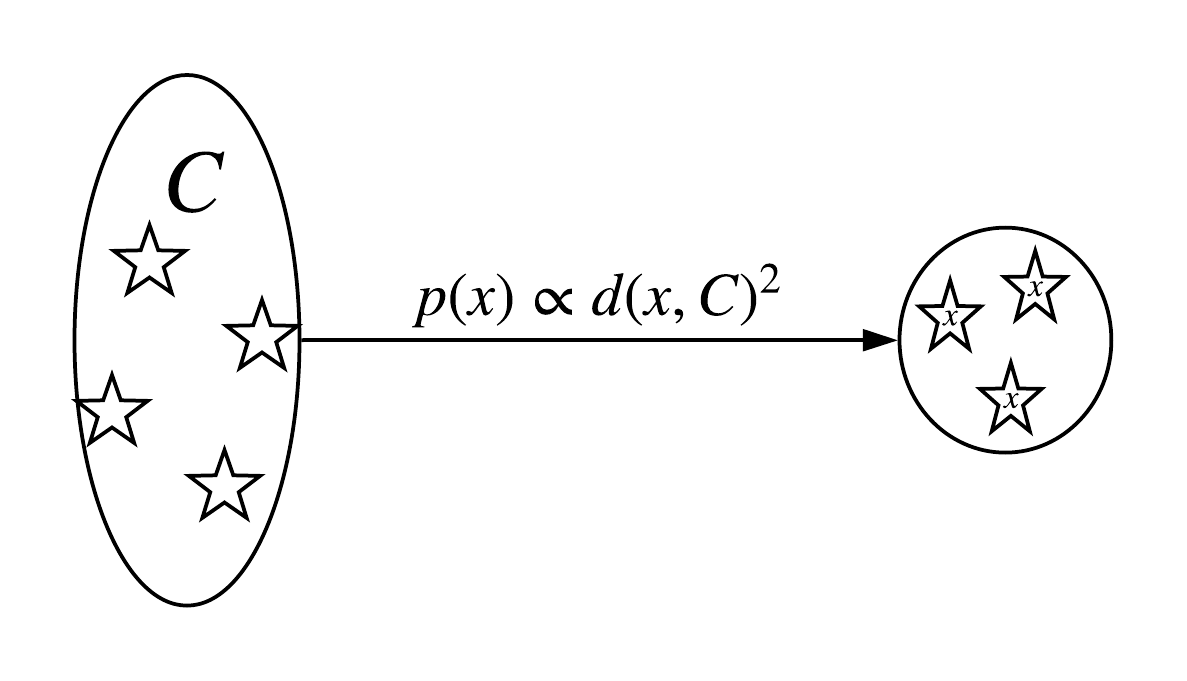
\includegraphics[scale=0.4]{kmeans||.png}
	\end{minipage}
	
\end{frame}

\begin{frame}{第一个贡献}
	将经典的$k$-­means++算法扩展到了带权的$k$-­means问题上并证明了扩展算法的聚类质量。
\end{frame}

\begin{frame}{带权$k$-means问题和新算法}
	\begin{definition}[带权$k$-means问题]
		\footnotesize
		给定数据集$\mathcal{X} \subseteq \R^d$和对应的权重$w$,找到一个大小为$k$的集合$C \subseteq \R^d$使得下面的目标函数最小。
		\begin{equation}
		\psi_C(\mathcal{X})=\sum_{x_i \in \mathcal{X}}w_i d^2(x_i,C)
		\end{equation}
	\end{definition}
	\vspace*{-0.5cm}
	\begin{center}
		\scalebox{0.7}{
			\begin{minipage}{0.78\linewidth}
				\begin{algorithm}[H]
					\caption{带权$k$-means++ seeding}
					\KwIn{数据集$\mathcal{X}$,权重$w$,类数目$k$}
					\KwOut{$k$个点$C$}
					$c_1 \gets $ 依概率$\frac{w_x}{\sum_{i \in \mathcal{X}} w_i}$从 $\mathcal{X}$中采样一个点\\
					$C \gets \{c_1\}$ \\
					\For{$i = 2,3, \ldots k$}{
						\For{$x \in \mathcal{X}$}{
							% we can calculate a small set of p instead of whole p(x)
							$p(x) \gets w_x\text{d}(x,C)^2/\sum_{x' \in \mathcal{X}} w_x'\text{d}(x',C)^2$
						}
						$x \gets$ 依分布$p$从$\mathcal{X}$中采样一个点\\
						$C \gets C\cup\{x\}$
					}
					\textbf{返回} $C$
				\end{algorithm}
			\end{minipage}
		}
	\end{center}
	
\end{frame}

\begin{frame}{带权$k$-means++的理论保证}
	\begin{theorem}[带权$k$-means++的理论保证]
		给定数据集$\mathcal{X}$和权重$w$,令$C$是带权$k$-means++返回的结果,则
		\begin{equation}
			\E[\psi_C(\mathcal{X})] \leq 8(\ln k + 2) \psi_\text{OPT}(\mathcal{X})
		\end{equation}
	\end{theorem}
	证明的框架:
	\begin{itemize}
		\item 考虑均匀采样的解的质量
		\item 考虑$d^2$ weighting的质量
		\item 用归纳法揭示中间解的关系
	\end{itemize}
\end{frame}

\begin{frame}{证明的框架}
	\begin{lemma}[均匀采样的解的质量]
		考虑任意最优类$A$,令$Z$是在$A$中以概率$\frac{w_z}{\sum_{i \in A} w_i}$被挑到的点,则, $\E[\psi_Z(A)] = 2 \psi_{\text{OPT}}(A)$
	\end{lemma}
	\begin{lemma}[$d^2$ weighting的质量]
		令$C$是任意中间结果,$1 \leq |C| \leq k-1$,令$A$是任意最优类,并且令$Z \in A$是基于$C$用$d^2$ weighting挑到的点,则,$\E[\psi_{C'}(A)|C,Z \in A] \leq 8 \psi_{\text{OPT}}(A)$,其中$C' = C \cup \{Z\}$
	\end{lemma}
\end{frame}

\begin{frame}{证明的框架}
%	\scalebox{0.8}{text}
	\begin{lemma}[中间解的关系]
		\footnotesize
		令$C$是任意中间结果,$1 \leq |C| \leq k-1$,任选$u>0$个“未覆盖”的最优类,令$\mathcal{X}_u$是那些类中的点,并且令$\mathcal{X}_c = \mathcal{X} - \mathcal{X}_u$,假定我们基于$C$用$d^2$ weighting的方法添加$0 \leq t \leq u$个点,令$C'$是添加后的解,则, 
		\begin{equation}
		\E[\psi_{C'}(\mathcal{X})|C] \leq [\psi_C(\mathcal{X}_c)+8\psi_{\text{OPT}}(\mathcal{X}_u)](1+H_t)+\frac{u-t}{u}\psi_C(\mathcal{X}_u)
		\end{equation}
		其中$H_t = 1+\frac{1}{2}+...+\frac{1}{t}$是调和数
	\end{lemma}
	\begin{figure}
		\centering
		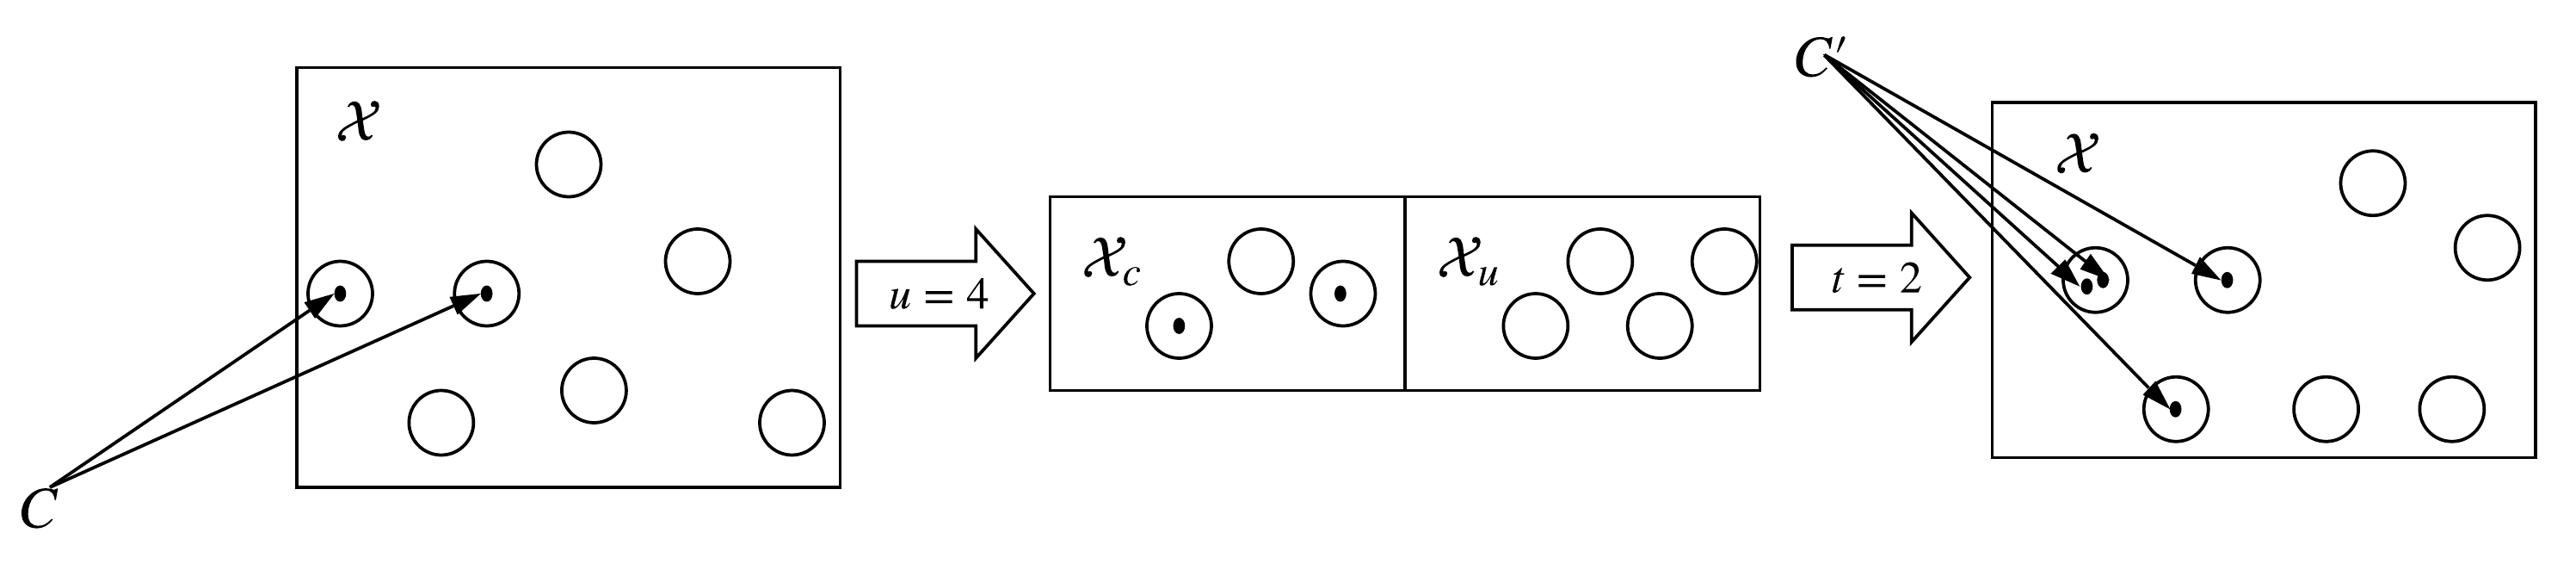
\includegraphics[scale=0.4]{lemma_relationships.png}
	\end{figure}
\end{frame}

\subsection{高效的算法}


\begin{frame}{基于均匀采样的聚类}
%	\begin{itemize}
%		\item reduce data size
%		\item uniform sampling works well
%	\end{itemize}
	\vspace*{-0.2cm}
	\begin{center}
		\scalebox{0.7}{\begin{algorithm}[H]
				\label{alg:clustering based on uni w/o}
				\caption{基于均匀采样的聚类}
				\KwIn{数据集$\mathcal{X}$,类数目$k$,采样数$s$,聚类算法$\mathcal{A}_c$}
				\KwOut{$k$个点$C$}
				$S \gets$ 均匀不放回采样$s$个点\\
				$C \gets$ 在$S$上用$\mathcal{A}_c$解决$k$-means问题\\
				\textbf{返回} $k$个点$C$
			\end{algorithm}}
		\scalebox{0.7}{
			\vbox{
				\begin{theorem}[算法\ref{alg:clustering based on uni w/o}的解的质量]
					令$0 < \delta <1/2$,$\alpha \geq 1$,$\beta >0$是近似系数,令$C$是均匀采样返回的解且$\mathcal{A}_c$是一个$\alpha$近似的算法,假定我们均匀不放回采样 $s$个点且
					\begin{equation}
					s \geq \ln(\frac{1}{\delta})(1+\frac{1}{n})/(\frac{\beta^2 m^2}{2\Delta^2 \alpha^2}+\frac{\ln(1/\delta)}{n})
					\end{equation}
					则,下式以至少$1-2\delta$的概率成立,
					\begin{equation}
					\phi_C(\mathcal{X}) \leq \textcolor{red}{4(\alpha + \beta)} \phi_\text{OPT}(\mathcal{X})
					\end{equation}
					其中$\Delta = \max\limits_{i,j}\norm{v_i - v_j}^2$是数据直径的平方,$m = \phi_\text{OPT}(\mathcal{X})/n$是最优目标函数值的平均值
				\end{theorem}
			}
		}
	\end{center}
\end{frame}

\begin{frame}{第二个贡献}
	\begin{itemize}
		\item 对均匀采样给出了一个更紧的理论界,并且证明在温和的数据假设下算法的运行时间在多项式对数级别
		\item 提出了新的Double-K-M$\text{C}^2$算法用于估计权重
		\item 给出了均匀采样、K-M$\text{C}^2$、Double-K-M$\text{C}^2$,和它们对应的kernel版本的MATLAB实现,用实验验证了这些算法的效率和有效性
	\end{itemize}
\end{frame}

\begin{frame}{一个更紧的理论界}
	\vspace*{-0.7cm}
	\begin{center}
		\scalebox{0.7}{
			\vbox{
				\begin{theorem}[均匀采样的更紧理论界]
					令$0 < \delta <1/2$,$\alpha \geq 1$,$\beta >0$是近似系数,令$C$是均匀采样返回的解且$\mathcal{A}_c$是一个$\alpha$近似的算法,假定我们均匀不放回采样 $s$个点且
					\begin{equation*}
					s \geq \ln(\frac{1}{\delta})(1+\frac{1}{n})/(\frac{\beta^2 m^2}{2\Delta^2 \alpha^2}+\frac{\ln(1/\delta)}{n})
					\end{equation*}
					则,下式以至少$1-2\delta$的概率成立,
					\begin{equation*}
					\phi_C(\mathcal{X}) \leq \textcolor{red}{(\alpha + \beta)} \phi_\text{OPT}(\mathcal{X})
					\end{equation*}
					其中$\Delta = \max\limits_{i,j}\norm{v_i - v_j}^2$是数据直径的平方,$m = \phi_\text{OPT}(\mathcal{X})/n$是最优目标函数值的平均值
				\end{theorem}
			}
		}
	\end{center}
	\vspace*{-0.3cm}
	\scriptsize
	证明的框架:
	\begin{enumerate}
		\item 说明$C$对于$S$会是一个好的解
		\item 如果$C$对于$\mathcal{X}$是一个坏的解,则大概率$C$对于$S$会是一个坏的解
		\item 根据1和2,说明$C$对于$\mathcal{X}$是一个好的解
	\end{enumerate}
\end{frame}

\begin{frame}{一个多项式对数时间的算法}
	假设数据是独立的从同一个分布$F$中采样出来的
	%todo which distributions satisfy these two assumptions?
	\begin{itemize}
		\item 分布$F$的尾部是指数衰减的,即$\exists c,t $使得$P[d(x,\mu(F))>a]\leq ce^{-at}$,其中$x\sim F$ 
		\item $F$在一个球面上的最大和最小概率密度的比值被一个大于等于1的常数限制(球面上的密度大于0)
	\end{itemize}
	\begin{theorem}[均匀采样的效率]
		\small
		令$0 < \delta <1/2$,$\alpha \geq 1$,$\beta >0$是近似系数,假定假设(A1)和(A2)成立,令令$C$是均匀采样返回的解,则,下式以至少$1-2\delta$的概率成立
		\begin{equation*}
		\phi_C(\mathcal{X}) \leq (\alpha + \beta)\phi_\text{OPT}(\mathcal{X})
		\end{equation*}
		如果采样$O(\ln(\frac{1}{\delta})\frac{\alpha^2}{\beta^2}k^2\log^4 n)$个点的话
	\end{theorem}
\end{frame}

\subsection{实验}

\begin{frame}{基准算法}
	\begin{itemize}
		\footnotesize
		\item 由于均匀采样既高效又有理论保证,我们设计实验来检验这一点
		\item 基准算法是K-M$\text{C}^2$ \citep{bachem2016approximate}和 Double-K-M$\text{C}^2$
		\item 由于$k$-means\(\vert \vert\)中的权重计算很花时间,我们提出一个新的称为Double-K-M$\text{C}^2$采样的算法来加速(估算权重)
	\end{itemize}
	\begin{center}
		\scalebox{0.7}{\begin{algorithm}[H]
				\caption{Double-K-M$\text{C}^2$采样}
				\KwIn{数据集$\mathcal{X}$,采样数$s$,游走步数$u$}
				\KwOut{$k$个点$C$}
				$S_1 \gets $ 在$\mathcal{X}$中用K-M$\text{C}^2$采样$s$个点\\
				$\mathcal{X}' \gets $ 在$\mathcal{X}$中移除$S_1$\\
				$S_2 \gets $ 在$\mathcal{X}'$中用K-M$\text{C}^2$采样$s$个点 \\
				对$S_1$中任意点$s_i$,令$w_i$是$S_2$中离$s_i$最近的点的数目 \\
				$C \gets$ 令$w_i+1$是$s_i$的权重,在带权$S_1$上运行一个$\alpha$近似算法 \\
				\textbf{返回} $k$个点$C$
			\end{algorithm}}
	\end{center}
	
\end{frame}

\begin{frame}{传统聚类}
	\begin{center}
		\scalebox{0.6}{
			\vbox{
				\begin{table}[H]
					\caption{数据量$n$,类数目$k$,维度$d$}
					\begin{tabular}{cccc}
						\toprule
						数据集 & $n$ & $k$ & $d$ \\
						\midrule
						a2 & 5250 & 35 & 2 \\
						a3 & 7500 & 50 & 2 \\
						b2-random-10 & 10000 & 100 & 2 \\
						b2-random-15 & 15000 & 100 & 2 \\
						b2-random-20 & 20000 & 100 & 2 \\
						\midrule
						KDD & 145751 & 200 & 74 \\
						RNA & 488565 & 200 & 8 \\
						Poker Hand & 1000000 & 200 & 10 \\
						\bottomrule
					\end{tabular}
				\end{table}
			}	
		}
	\end{center}
	\begin{itemize}
		\scriptsize
		% todo Lloyd algorithm iterations?
		\item 游走步数: $u=200$
		\item 采样量: Double-K-M$\text{C}^2$和均匀采样分别是$1.5 \log^2 n$和$0.7 \log^4 n$
		\item $\alpha$近似算法:(带权)$k$-means++接Lloyd
		\item 评价指标:距离计算次数和$k$-means目标函数
	\end{itemize}
\end{frame}

\begin{frame}{结果}
	\begin{minipage}{0.4\linewidth}
		\scriptsize
		\begin{enumerate}
			\item 均匀采样差不多比K-M$\text{C}^2$慢10倍,不过随着数据的增多时间增长较慢,目标函数值差不多是K-M$\text{C}^2$的60\%
			\item Double-K-M$\text{C}^2$比K-M$\text{C}^2$聚类质量好时间花费比均匀采样少
			\item 如果你想要一个好的聚类质量且时间花费要合理的话,选择Double-K-M$\text{C}^2$,如果追求质量,推荐均匀采样
		\end{enumerate}
	\end{minipage}
	\scalebox{0.55}{
		\begin{minipage}{1.0\linewidth}
			\begin{figure}[H]
				\centering
				\begin{subfigure}{0.47\linewidth}
					\centering
					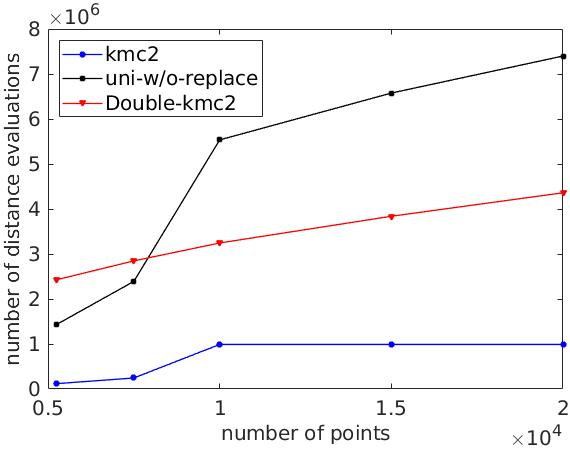
\includegraphics[width=\linewidth]{syn-running-time.jpg}
					\caption{\small{合成数据集上的距离计算次数}}
					\label{}
				\end{subfigure}
				\hfill
				\begin{subfigure}{0.47\linewidth}  
					\centering 
					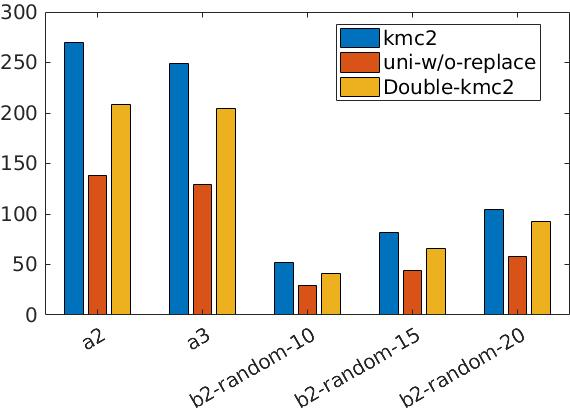
\includegraphics[width=\linewidth]{syn-sum-squared-distances.jpg}
					\caption{\small{合成数据集上的$k$-means目标函数值}}
					\label{}
				\end{subfigure}
				\vskip\baselineskip
				\begin{subfigure}{0.47\linewidth}   
					\centering 
					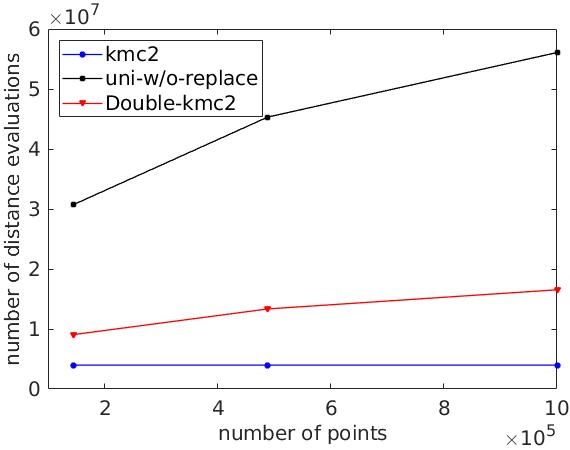
\includegraphics[width=\linewidth]{real-running-time.jpg}
					\caption{\small{真实数据集上的距离计算次数}}    
					\label{}
				\end{subfigure}
				\hfill
				\begin{subfigure}{0.47\linewidth}
					\centering 
					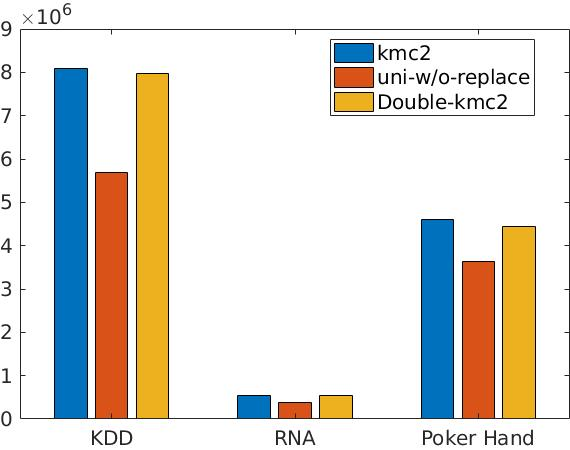
\includegraphics[width=\linewidth]{real-sum-squared-distances.jpg}
					\caption{\small{真实数据集上的$k$-means目标函数值}}    
					\label{}
				\end{subfigure}
				\caption{$k$-means目标函数值和时间花费随数据量变化图}
				\label{fig:running time & sum of distances}
			\end{figure}
		\end{minipage}
%		\vbox{
%			
%		}
	}
	
\end{frame}

\begin{frame}{图像分割}
	\begin{center}
		\scalebox{0.7}{
			\vbox{
				\begin{table}[H]
					\caption{数据量$n$,类数目$k$}
					\begin{tabular}{ccc}
						\toprule
						数据集 & $n$ & $k$ \\
						\midrule
						baby & 900(30 * 30) & 5 \\
						kitten & 3600(60 * 60) & 5 \\
						bear & 14400(120 * 120) & 5 \\
						\bottomrule
					\end{tabular}
				\end{table}
			}
		}
	\end{center}
	\begin{itemize}
		\scriptsize
		\item 均匀采样、Double-K-M$\text{C}^2$,和K-M$\text{C}^2$的kernel版
		\item 用\citet{stella2003multiclass}的方法计算相似度矩阵$A$,寻找离$A$最近的正定矩阵$K$做为kernel
		\item 游走步数:$u=200$
		\item 采样量:Double-K-M$\text{C}^2$和均匀采样分别是$0.25\log^2 n$和$0.4\log^4 n$
		\item $\alpha$近似算法:(带权)kernel $k$-means++接kernel Lloyd
		\item 评价指标:距离计算次数和kernel $k$-means目标函数值
	\end{itemize}
\end{frame}

\begin{frame}{结果}
	\begin{minipage}{0.4\linewidth}
		\scriptsize
		\begin{enumerate}
			\item 均匀采样的kernel版有最优的聚类质量而时间开销增长不快
			\item Double-K-M$\text{C}^2$的kernel版有着和均匀采样差不多的聚类质量而时间开销少很多
			\item 因此,如果追求聚类质量,推荐使用Double-K-M$\text{C}^2$,如果要更快的速度,K-M$\text{C}^2$是一个更好的选择
		\end{enumerate}
	\end{minipage}
	\scalebox{0.55}{
		\begin{minipage}{1.0\linewidth}
			\begin{figure}[H]
				\centering
				\begin{subfigure}{0.493\columnwidth}   
					\centering 
					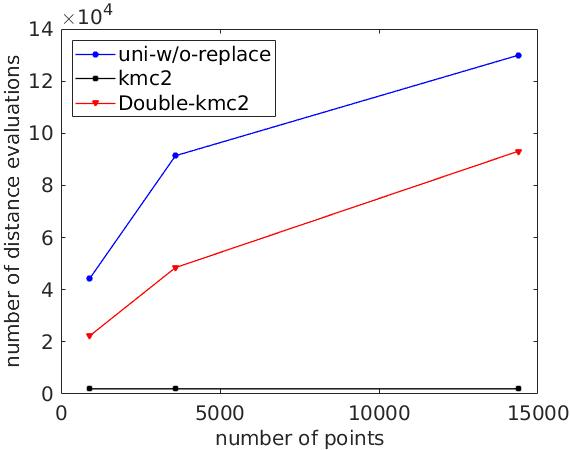
\includegraphics[width=\linewidth]{image-running-time.jpg}
					\caption{图片数据上的距离计算次数}
				\end{subfigure}
				%	    \begin{minipage}{0.494\columnwidth}
				%	        \centering
				%	        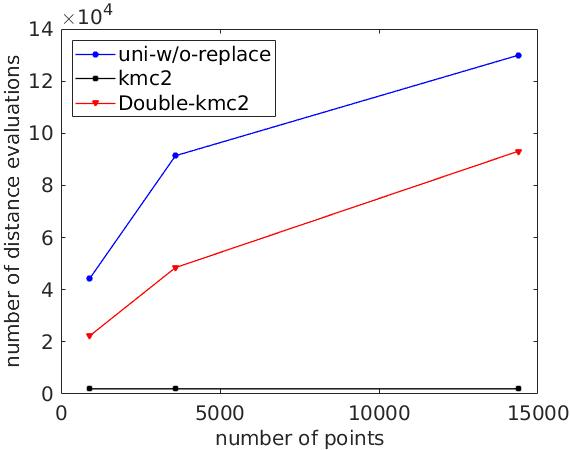
\includegraphics[width=\linewidth]{image-running-time.jpg}
				%	    \end{minipage}
				%	    \hfill
				\begin{subfigure}{0.493\columnwidth}   
					\centering 
					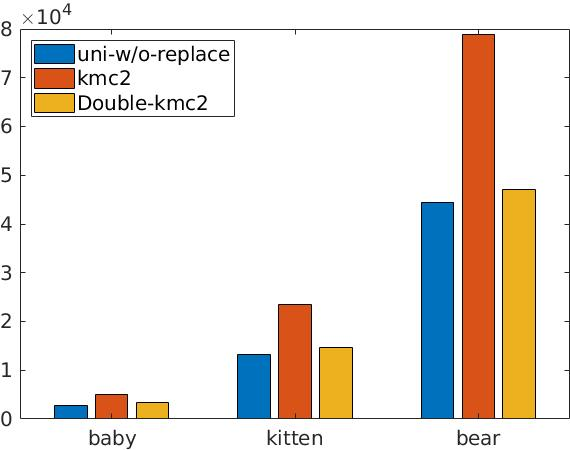
\includegraphics[width=\linewidth]{image-obj.jpg}
					\caption{图片数据上的kernel $k$-means目标函数值}
				\end{subfigure}
				
				%	    \begin{minipage}{0.494\columnwidth}
				%	        \centering
				%	        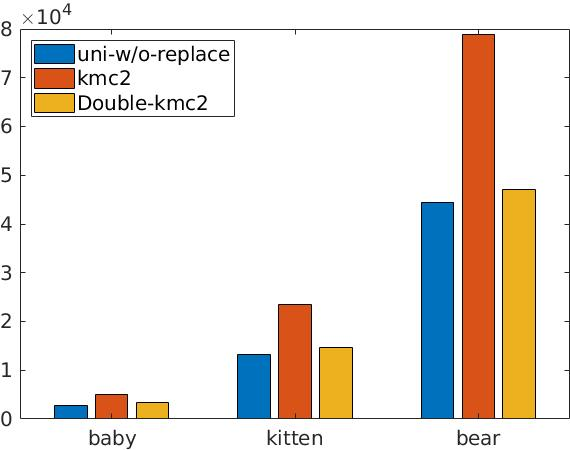
\includegraphics[width=\linewidth]{image-obj.jpg}
				%	    \end{minipage}
				
%				\caption{(Left) . (Right) }
				\caption{kernel $k$-means目标函数值和时间开销随数据量变化图}
				\label{fig: image running time & ncut}
			\end{figure}
		\end{minipage}
		%		\vbox{
		%			
		%		}
	}
	
\end{frame}

\section{谱聚类}

\subsection{背景}

\begin{frame}{谱聚类问题}
	\begin{itemize}
		\item 此问题的来源之一是图论
		\item 该问题也是NP难的
	\end{itemize}
	\begin{definition}[Normalized Cut]
		记$v_i$是节点$i$,$C_j$是类$j$,找到一个划分矩阵$F_{ij} = \begin{cases} 1 & {v_i \in C_j} \\ 0 & {otherwise}
		\end{cases}$使得下面的目标函数能最小
		\begin{equation}
			\min\limits_{F} \operatorname{Tr}(\frac{F^T L F}{F^T D F})
		\end{equation}
		其中$L = D-A$,$A$图的相似度矩阵,$D$是$A$的度矩阵
	\end{definition}
\end{frame}

\subsection{有理论保证且高效的算法}

\begin{frame}{转变为传统聚类}
	\footnotesize{
		\begin{definition}[带权kernel $k$-means问题]
			给定数据集$\mathcal{X} \subseteq \R^d$和对应权重$w$以及一个映射函数$\varphi(.)$,找到一个大小为$k$的集合$C$使得下面的目标函数最小
			\begin{equation}
			\Psi_C(\mathcal{X}) = \sum_{i=1}^k \sum_{x_j \in \pi_i}w_j \norm{\varphi(x_j)-C_i}^2
			\end{equation}
			其中$\pi_i$表示第$i$个类,$\cup_{i=1}^k \pi_i = \mathcal{X}$, $C_i = \frac{\sum_{x_j \in \pi_i}w_j \varphi(x_j)}{\sum_{j \in \pi_i}w_j}$
		\end{definition}
	}
	\footnotesize{
		\begin{lemma}[两种聚类间的关系]
			令$W$和$K$是带权kernel $k$-means问题的权重和核矩阵,令$W=D$且$K=D^{-1}AD^{-1}$,其中$D$和$A$是谱聚类的度矩阵和相似度矩阵,则,
			\begin{equation}
			\Psi_C(\mathcal{X})=\operatorname{Tr}(D^{-1/2}AD^{-1/2})-k+Ncut
			\end{equation}
		\end{lemma}
	}
	
\end{frame}

\begin{frame}{基于均匀采样的算法}
	\vspace*{-0.25cm}
	\begin{center}
		\scalebox{0.67}{\begin{algorithm}[H]
				\SetNoFillComment
				\caption{基于均匀采样和带权kernel $k$-means的谱聚类算法\citep{Mohan:2017:BNA:3172077.3172235}}\label{alg: uniform_wkk}
				\KwIn{数据集$\mathcal{X}$,类数目$k$,采样数$s$,相似度矩阵$A$,度矩阵$D$}
				\KwOut{$\mathcal{X}$的$k$个类的划分}
				$S \gets$ 均匀不放回的从$1,2,...,n$采样$s$个数字\\
				$W \gets D,K \gets D^{-1}AD^{-1}$\\
				$W_s \gets W(S,S), K_s \gets K(S,S)$\\
				$\pi' \gets$ 给定$W_s$和$K_s$在采样点上运行一个$\alpha$近似算法\\
				\tcc{把数据点靠到对应的中心点上}
				\For{$i = 1,...,n$}{
					\For{$c = 1,...,k$}{
						\begin{equation*}
						d(a_i,m_c) \gets K_{i i}-\frac{2 \sum_{a_{j} \in \pi'_{c}} w_{j} K_{i j}}{\sum_{a_{j} \in \pi'_{c}} w_{j}}+\frac{\sum_{a_{j}, a_{l} \in \pi'_{c}} w_{j} w_{l} K_{j l}}{\left(\sum_{a_{j} \in \pi'_{c}} w_{j}\right)^{2}}
						\end{equation*}\\
					}
					$j \gets \argmin\limits_{c = 1,2,...,k} d(a_i,m_c)$\\
					$Y_{ij} \gets 1$
				}
				\textbf{返回} $Y$
			\end{algorithm}}
		\end{center}
\end{frame}

\begin{frame}{第三个贡献}
	\begin{itemize}
		\item 对基于均匀采样和带权kernel $k$-means的谱聚类给出了更紧的理论界
		\item 给出了这一算法的MATLAB实现,并用实验验证了它的效率和解的质量
	\end{itemize}
\end{frame}

\begin{frame}{一个更紧的理论界}
	\begin{theorem}[算法\ref{alg: uniform_wkk}的更紧理论界]
		Let $0 < \delta <1/2$, $\alpha \geq 1$, and $\beta >0$ be approximation parameters. Suppose we sample $s$ points in Algorithm \ref{alg: uniform_wkk} such that,
		\begin{equation}
		s \geq \ln(\frac{1}{\delta})(1+\frac{1}{n})/(\frac{\beta^2 m^2}{2\Delta^2 \alpha^2}+\frac{\ln(1/\delta)}{n})
		\end{equation}
		we have
		\begin{equation}
		Ncut \leq \textcolor{red}{(\alpha + \beta)} Ncut^* + (\alpha + \beta -1)c
		\end{equation}
		with probability at least $1-2\delta$, where $\Delta = \max\limits_{i,j}\norm{\varphi(x_i) - \varphi(x_j)}^2$ is the squared diameter of the data in the mapped space, $m = \Psi_\text{OPT}(\mathcal{X})/n$ is the average of the optimal objective, $c$ is a constant irrelevant to partitions, $Ncut^*$ is the optimal $Ncut$.
	\end{theorem}
\end{frame}

\subsection{实验}

\begin{frame}{传统聚类}
	\begin{center}
		\scalebox{0.7}{
			\vbox{
				\begin{table}[H]
					\caption{data size $n$, number of clusters $k$, dimension $d$}
					\label{tab:datasets_spectral_clustering}
					\begin{tabular}{ccccc}
						\toprule
						datasets & name & $n$ & $d$ & $k$ \\
						\midrule
						$D_1$ & segment &2310 & 19 & 7 \\
						$D_2$ & MnistData-05 &3495 &784 & 10 \\
						$D_3$ & MnistData-10 &6996 & 784 & 10 \\
						$D_4$ & isolet5 &7797 & 617 & 26 \\
						$D_5$ & USPS &9298 & 256 & 10 \\
						$D_6$ & letter-recognition &20000 & 16 & 26 \\
						\bottomrule
					\end{tabular}
				\end{table}
			}	
		}
	\end{center}
	\begin{itemize}
		\scriptsize
		\item Experiments will be performed to verify the efficiency and the effectiveness of uniform sampling
		\item algorithms: weighted kernel $k$-means(uniform sampling vs no-sampling)
		\item anchor based graph construction method
		\item sampling size: 20\% of data points
		\item $\alpha$ approximation algorithm: weighted kernel $k$-means++
		\item evaluation metrics: time(s) and Ncut
	\end{itemize}
\end{frame}

\begin{frame}{结果}
	\begin{minipage}{0.4\linewidth}
		\scriptsize
		\begin{enumerate}
			\item The sampling version is about 20$\sim$50 times faster than the no-sampling one while Ncut is not larger than the no-sampling version by 25\%
			\item Hence, the uniform sampling method is a good choice for its amazing efficiency and reasonable clustering quality.
		\end{enumerate}
	\end{minipage}
	\scalebox{0.57}{
		\begin{minipage}{1.0\linewidth}
			\begin{figure}[H]
				\begin{subfigure}{.49\linewidth}
					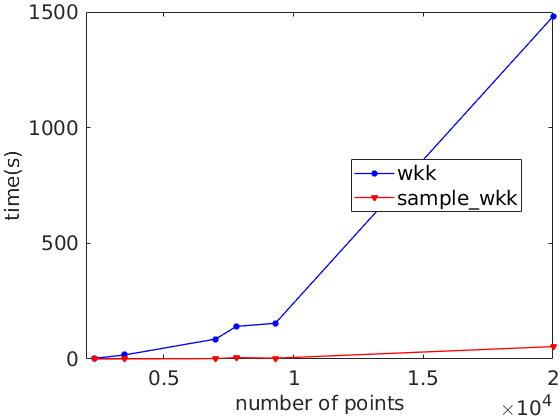
\includegraphics[width=\linewidth]{sp-running_time.jpg}
					\caption{time costs(s)}
				\end{subfigure}
				\begin{subfigure}{.49\linewidth}
					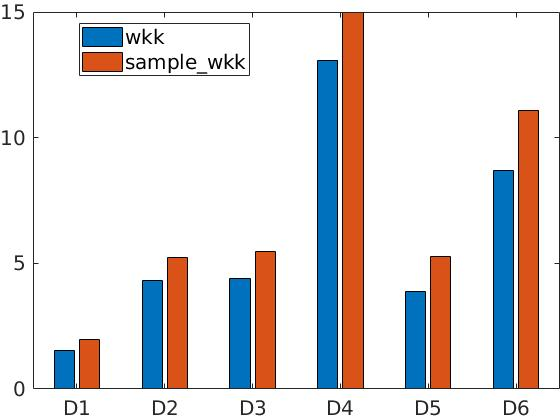
\includegraphics[width=\linewidth]{sp-Ncuts.jpg}
					\caption{Ncut}
				\end{subfigure}
				\caption{results of spectral clustering}
				\label{fig: sp-experiments}
			\end{figure}
		\end{minipage}
		%		\vbox{
		%			
		%		}
	}
	
	
	
\end{frame}

\section{贡献总结}

\begin{frame}{总结}
	\begin{enumerate}
		\small
		\item (Theoretical) The classic $k$-­means++ algorithm has been extended to weighted $k$-­means problem and proofs on the clustering quality are given.
		\item (Theoretical) A sharper bound for the uniform sampling algorithm on $k$-means is proved, and a further proof indicates that this algorithm runs in polylogarithmic time given mild assumptions on datasets.
		\item (Theoretical) A sharper bound for the spectral clustering is proved.
		\item (Empirical) We give MATLAB implementations of uniform sampling, K-M$\text{C}^2$, Double-K-M$\text{C}^2$, and their corresponding kernel versions on $k$-means. Experiments validate the efficiency and effectiveness of these algorithms.
		\item (Empirical) We give MATLAB implementations of the weighted kernel $k$-means based spectral clustering algorithm and its corresponding sampling versions. Experiments are used to justify these algorithms on the efficiency and solution quality.
	\end{enumerate}
\end{frame}

% reference:
% https://tex.stackexchange.com/questions/86101/beamer-creating-a-slide-with-short-centered-prominent-text
\begin{frame}[plain,c]
\begin{center}
\Huge 问题?
\end{center}
\end{frame}

\begin{frame}{参考文献}
	\scriptsize
    \bibliographystyle{unsrt}
    \bibliography{bibfile}
\end{frame}

\clearpage\end{CJK*}
\end{document}
